En la sección \coloredUnderline{\hyperlink{sec:6_1-Identificacion_actores}{\ref*{sec:6_1-Identificacion_actores} \nameref*{sec:6_1-Identificacion_actores}}} se identificaron los actores del sistema,
cada uno con niveles de acceso y funcionalidades específicas adecuadas a su rol dentro de la plataforma. 

En este apartado se detalla el diagrama de navegabilidad de cada uno de los actores identificados en la sección mencionada anteriormente.
Para cada actor se detallan las vistas a las que puede acceder.

Las cajas que aparecen sombreadas en el diagrama representan las vistas que son accesibles desde cualquier otra vista,
debido a que se encuentran bien en el menú de navegación o en el pie de página de la aplicación.

La vista \textit{Home} es la vista principal de la aplicación, en función de si el usuario está autenticado o no, tendrá
una funcionalidad u otra, pero siempre es el punto de partida de la navegación y accesible desde cualquier vista.


\subsubsection{Usuario no autenticado}
En la \coloredUnderline{\hyperlink{fig:navegabilidad-usuario-no-autenticado}{Figura \ref*{fig:navegabilidad-usuario-no-autenticado}}} se muestra el diagrama de navegabilidad del usuario no autenticado.

\begin{figure}[H]
    \centering
    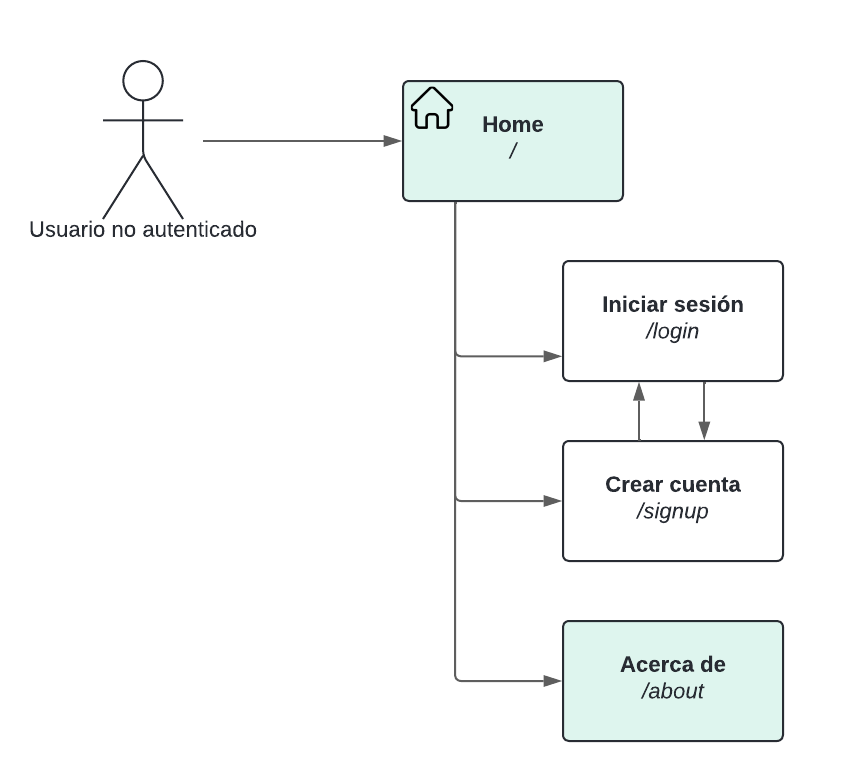
\includegraphics[width=0.5\textwidth]{figures/6-Analisis/6-Interfaz/navegabilidad-guest.png}
    \caption{Diagrama de navegabilidad del usuario no autenticado.}
    \hypertarget{fig:navegabilidad-usuario-no-autenticado}{}
    \label{fig:navegabilidad-usuario-no-autenticado}
\end{figure}

\subsubsection{Usuario autenticado}
En la \coloredUnderline{\hyperlink{fig:navegabilidad-usuario-autenticado}{Figura \ref*{fig:navegabilidad-usuario-autenticado}}} se muestra el diagrama de navegabilidad del usuario autenticado.

\begin{figure}[H]
    \centering
    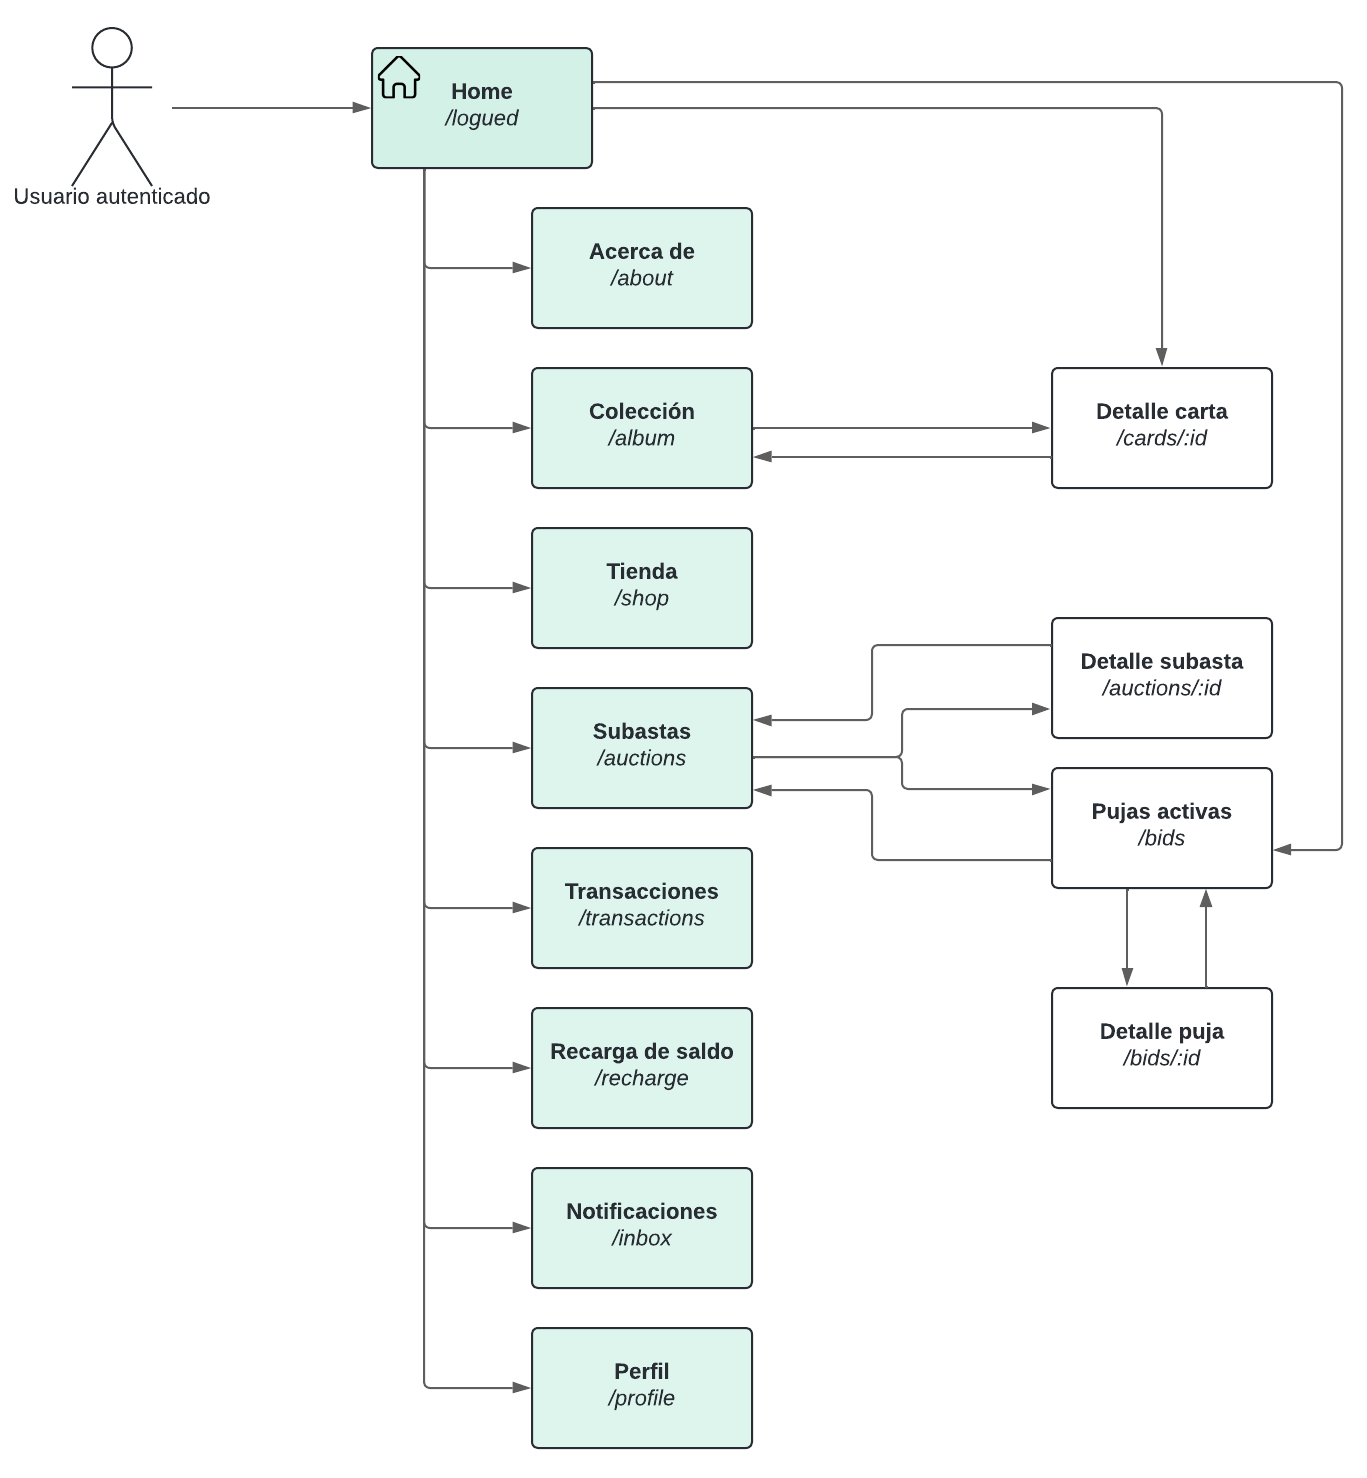
\includegraphics[width=0.8\textwidth]{figures/6-Analisis/6-Interfaz/navegabilidad-standard.png}
    \caption{Diagrama de navegabilidad del usuario autenticado.}
    \hypertarget{fig:navegabilidad-usuario-autenticado}{}
    \label{fig:navegabilidad-usuario-autenticado}
\end{figure}

\subsubsection{Administrador}
En la \coloredUnderline{\hyperlink{fig:navegabilidad-administrador}{Figura \ref*{fig:navegabilidad-administrador}}} se muestra el diagrama de navegabilidad del administrador.

\begin{figure}[H]
    \centering
    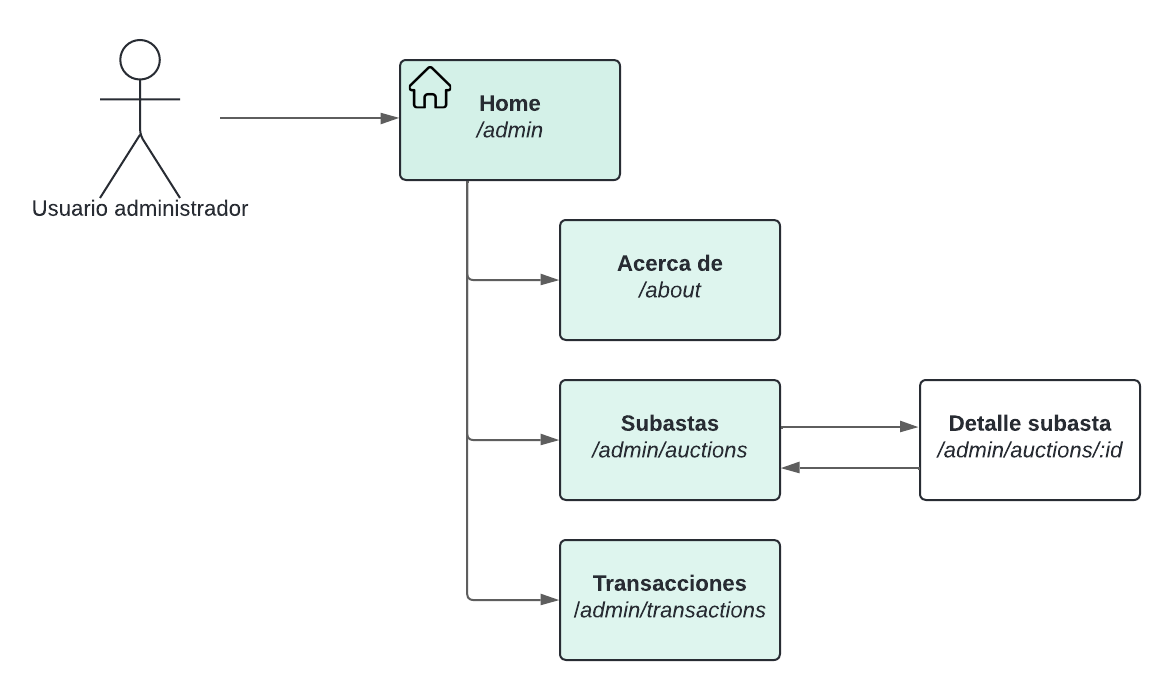
\includegraphics[width=0.6\textwidth]{figures/6-Analisis/6-Interfaz/navegabilidad-admin.png}
    \caption{Diagrama de navegabilidad del administrador.}
    \hypertarget{fig:navegabilidad-administrador}{}
    \label{fig:navegabilidad-administrador}
\end{figure}